\chapter{Fundamentação teórica}
\label{cap:fundamentacao-teorica}

Neste capítulo, a fundamentação teórica das tecnologias abordadas neste trabalho é realizada. Conceitos básicos sobre a linguagem de programação Java são mostrados, abordando tanto os pilares da orientação a objetos presente na linguagem quanto bibliotecas relevantes para as aplicações desenvolvidas na área. Posteriormente, conceitos relevantes para a o desenvolvimento de interfaces de usuário (\textit{user interface}, UI) são apresentados, apontando características e ferramentas utilizada no processo de construção de interfaces.

\section{Java}
\label{sec:java}

Uma das tecnologias presentes no Programa de Estágio Jedi Internship e abordadas nesse trabalho corresponde ao aprendizado e aplicação de conceitos da linguagem de programação Java. Originada inicialmente em 1991 com o codinome de Oak, e nomeada de Java somente em 1995, atualmente a linguagem é uma das mais utilizadas na área de Computação, sendo administrada pela empresa Oracle e estando em sua oitava versão~\cite{ocastudyguide-2015}.

Em suas primeiras versões, o propósito inicial do Java era conectar diferentes tipos de micro-sistemas da empresa Sun, sendo uma linguagem comum entre eles. A habilidade de escrever um código que pode funcionar em mais de um sistema é conhecida como \textit{write once, run anywhere} (WORA), sendo uma das principais características da linguagem. Ao escrever um código em Java, o compilador Javac processa o arquivo fonte para um arquivo em \textit{bytecode}, e um interpretador JVM específico para a plataforma se encarrega de processar esse arquivo posteriormente, como mostrado na Figura~\ref{fig:java-fluxo}~\cite{ocastudyguide-2015}.

\begin{figure}[htb!]
  \centering
  \caption{Esquema de execução de um código escrito em Java.}
  \label{fig:java-fluxo}
  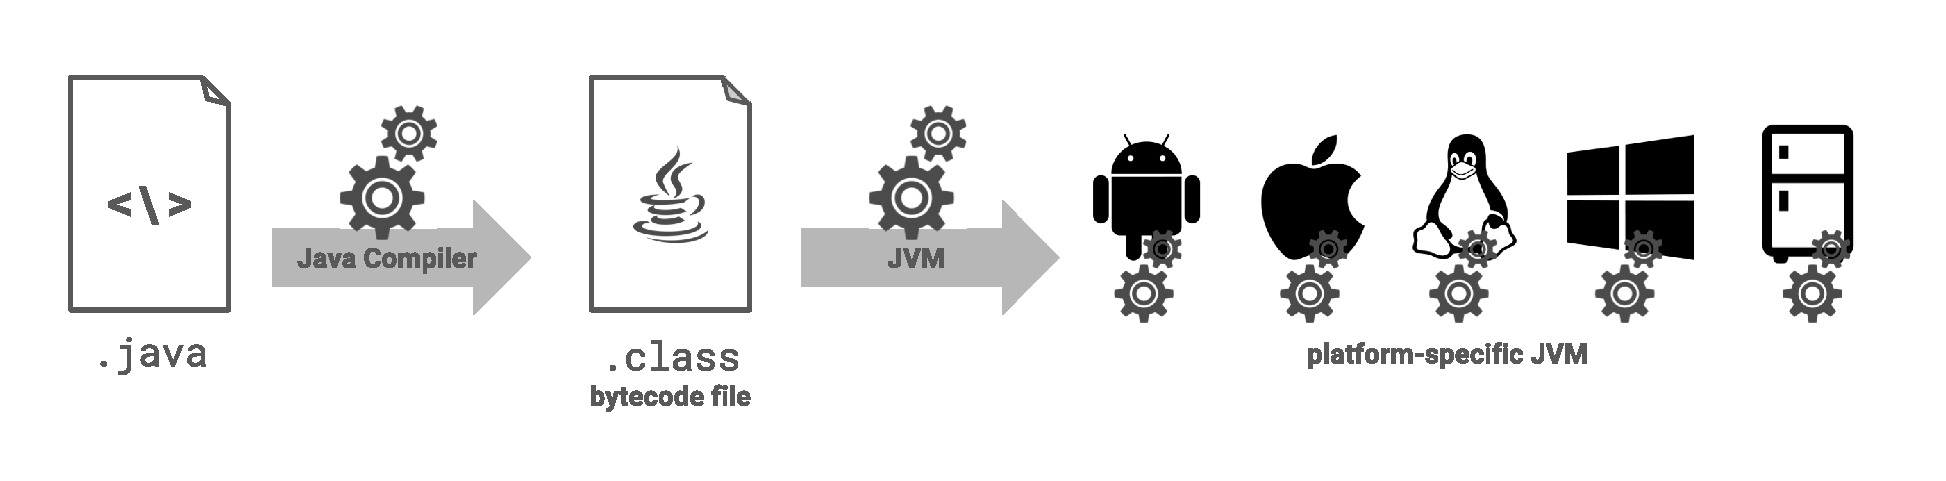
\includegraphics[width=\textwidth, keepaspectratio=true]{img/java-fluxo}
  \fonte{Próprio autor.}
\end{figure}

Além do WORA, outra característica marcante da linguagem é a implementação do conceito de orientação a objetos. Para implementar tal conceito, o Java faz uso de classes e objetos: enquanto uma classe funciona como uma especificação de uma ideia, um objeto corresponde a uma instância, uma materialização dessa ideia, sendo que uma classe pode possuir vários objetos instanciados~\cite{ocastudyguide-2015}.

A relação entre classes e objetos dá margem para diversos outros conceitos presentes na linguagem Java. O conceito de encapsulamento, por exemplo, faz uso de modificares de acesso nos atributos e métodos de cada classe para controlar quais objetos podem acessá-los, enquanto o conceito de herança entre as classes determina uma relação de pai-filho entre elas, tornando possível que uma herde atributos e métodos da outra~\cite{ocastudyguide-2015}.

Conceitos de abstração, composição e interfaces também estão presentes na linguagem, possibilitando a criação de classes não instanciáveis, classes compostas por diversos objetos, e a garantia que alguns métodos são implementados em determinadas classes, respectivamente. Por fim, um conceito essencial da linguagem é o polimorfismo, que permite que um objeto seja referenciado por diversas maneiras, como por meio das classes que ele herda, ou de interfaces que implementa~\cite{ocastudyguide-2015}.

Além dos conceitos apresentados, o Java ainda conta com bibliotecas como o \textit{collections framework}, que implementam diferentes estruturas de dados utilizadas comumente na programação de computadores. Estruturas como \textit{hashes}, listas de vetores, pilhas e filas podem ser utilizadas através das interfaces \verb|HashSet|, \verb|ArrayList|, \verb|Stack| e \verb|Queue|, respectivamente. Além de eliminar a necessidade do programador construir cada uma das estruturas, a utilização delas é extremamente comum em aplicações construídas em Java, facilitando o trabalho do desenvolvedor~\cite{javacollections-2001}.

Tanto os elementos presentes no \textit{collections framework} quanto os conceitos apresentados previamente podem ser utilizados para diversos tipos de aplicações em Java~\cite{javacollections-2001}. O gerenciamento de banco de dados relacionais em Java, por exemplo, utiliza uma interface de programação de aplicações (\textit{application programming interface}, API) chamada Java Database Connectivity (JDBC). O JDBC abstrai a implementação de banco de dados específicos, criando uma camada única que contribui para a implementação de métodos para estabelecer conexões, criar \textit{queries} de acesso, e extrair resultados de buscas, por exemplo~\cite{databaseprogramming-2000}.

O JDBC ainda conta com maneiras para gerenciar múltiplas conexões em um servidor através de um \textit{pool} de conexões, e de centralizar o acesso de dados por meio de objetos de acesso a dados (\textit{data access object}, DAO)~\cite{databaseprogramming-2000}. A utilização de alguns desses recursos é aprofundada na Seção~\ref{sec:java-atividades} do Capítulo~\ref{cap:atividades-desenvolvidas}, que descreve as atividades realizadas durante a área de Java do Programa de Estágio, focando na utilização da linguagem atrelada ao \textit{backend} de sistemas.

\section{Desenvolvimento de interfaces de usuário}
\label{sec:ui}

Uma das principais tarefas na construção do \textit{frontend} de um sistema é o desenvolvimento de interfaces de usuário (\textit{user interfaces}, UI). No desenvolvimento de uma aplicação Web, o designer de interfaces cria interfaces gráficas guiado por um designer de experiência de usuário (\textit{user experience}, UX), e passa as interfaces prontas para o desenvolvedor UI. Em posse das telas, cabe ao desenvolvedor transformá-las em código, o que ocorre essencialmente por meio da combinação de três tecnologias diferentes: a Linguagem de Marcação de Hipertexto (\textit{Hyper Text Markup Language}, HTML), as Folhas de Estilo em Cascata (\textit{Cascading Stylesheets}, CSS) e a linguagem de programação de propósito geral JavaScript~\cite{oppermann-2002, stefaner-2009}.

Para desenvolver as interfaces de usuário, é necessário primeiro construir a estrutura da página Web que irá abrigá-las, o que é feito por meio do HTML. O HTML dá estrutura para uma página Web, declarando formulários, \textit{links}, botões e outros elementos que possam estar presentes na interface por meio de \textit{tags}. Cada \textit{tag} pode ter uma gama de atributos – botões, por exemplo, podem ter alguma ação disparada quando são clicados por meio do atributo \verb|onClick|. Cada \textit{tag} é representada graficamente por diferentes \textit{browsers} de uma formas distintas, e utiliza-se então o CSS para dar um estilo próprio e único a cada um dos elementos~\cite{oppermann-2002, stefaner-2009}.

O CSS possibilita a estilização de diversas propriedades de cada elemento, como cores, tipografia, posicionamento e disposição na tela. Ainda é possível estilizar os elementos em diferentes estados que eles possam se encontrar, como quando o mouse os clica ou quando somente passa sobre eles. Além disso, é possível estilizar um grupo de elementos baseado em relações de hierarquia por meio de seletores CSS. Também é comum a utilização de pré-processadores de CSS como o SASS, que incluem a utilização de variáveis e uma sintaxe simplificada, por exemplo, para aumentar o desempenho e extender as funcionalidades do CSS~\cite{stefaner-2009}.

Por fim, o JavaScript é uma linguagem de programação de propósito geral que busca dar dinamismo para as páginas Web. Por meio dessa linguagem, é possível configurar as ações provenientes do disparo do botão mencionadas anteriormente, além de modificar o comportamento de elementos da página. Embora seja possível desenvolver interfaces de usuário somente por meio das três tecnologias, pode-se fazer uso de algum \textit{framework} JavaScript durante esse processo, como o AngularJS~\cite{angularjs-2017, oppermann-2002}.

O AngularJS é um \textit{framework} JavaScript que busca simplificar o desenvolvimento Web, possibilitando a utilização de uma arquitetura \textit{Model-View-Controller} (MVC) em uma aplicação Web. Criado por Hevery e Abrons em 2009, o \textit{framework} hoje encontra-se na versão 1.7, possuindo ainda uma versão 2 em fase de testes. Por meio do AngularJS, é possível conectar os dados exibidos na interface com um modelo constituído de variáveis e um controlador codificado em JavaScript que define métodos e lógica para a interface. A essa conexão dá-se o nome de \textit{data binding}, e uma das principais características do \textit{framework} em sua primeira versão é possibilitar o \textit{two-way data binding}, isso é, ocorre a conexão tanto do modelo com a interface quanto da interface com o modelo~\cite{angularjs-2017}.

Além do \textit{data binding}, o AngularJS também disponibiliza outras funcionalidades a fim de aumentar o dinamismo em aplicações Web, como diretivas, templates e filtros que podem ser incorporados diretamente no HTML por meio de atributos ou dentro de um arquivo JavaScript que contenha a lógica da interface~\cite{angularjs-2017}. Todas essas funcionalidades contribuem para o desenvolvimento de um projeto legível, com fácil manutenção e reutilização de código, sendo todas elas utilizadas nas atividades realizadas durante a área de UI do Programa de Estágio, mostrada na Seção~\ref{sec:ui-atividades} desse trabalho.